\documentclass[12pt,a4paper]{article}
\usepackage{amsmath,amsfonts,amssymb}
\usepackage{graphicx}
\usepackage{enumitem}
\usepackage[dvipsnames]{xcolor}
\usepackage{pgfplots}
\usepackage{hyperref}
\usepackage{soul}
\usepackage{framed}
\usepackage{booktabs} 
\usepackage{tabularx}
\usepackage{array}


\definecolor{lessonbgcolor}{rgb}{0.9,0.9,1}
\definecolor{examplecolor}{rgb}{0.8,1,0.8}
\definecolor{noteboxcolor}{rgb}{1,0.8,0.8}
\newenvironment{lesson}[1]
  {\begin{framed}\colorbox{lessonbgcolor}{
  \parbox{\dimexpr\linewidth-2\fboxsep}{
  \textbf{#1}}}\end{framed}}
  
\newenvironment{example}
  {\begin{framed}\colorbox{examplecolor}{
  \parbox{\dimexpr\linewidth-2\fboxsep}{
  \textbf{Example:}}}}
  {\end{framed}}
\newenvironment{note}
  {\begin{framed}\colorbox{noteboxcolor}{
  \parbox{\dimexpr\linewidth-2\fboxsep}{
  \textbf{Note:}}}}
  {\end{framed}}

\pgfplotsset{width=7cm,compat=1.17}
\title{Grade 11 Functions Notes: Unit 1}
\author{Kensukeken}
\date{September 2023}

\begin{document}
\maketitle

\section*{Unit 1: Intro To Functions}

\subsection*{Lesson 1 - Domain and Range}
The domain and range of a function describe the possible input and output values, respectively.



\textbf{\hl{Example 1:}} For \(f(x) = \sqrt{x}\), the domain is \(x \geq 0\) since you can't take the square root of a negative number without delving into complex numbers.

\textbf{\hl{Example 2:}} For \(f(x) = \frac{1}{x}\), the domain is \(x \neq 0\) since division by zero is undefined.

\textbf{\hl{Example 3:}} For a parabola \(f(x) = x^2\), the range is \(f(x) \geq 0\).

\subsection*{Lesson 2 - Function Notation}
Function notation introduces a more concise way to represent equations.

\textbf{\hl{Example 1:}} Given \(f(x) = 2x^2 + 3\), find \(f(2)\). Solution: \(f(2) = 2(2^2) + 3 = 11\).

\textbf{\hl{Example 2:}} If \(f(x) = x + 5\), what is \(f(3)\)? Solution: \(f(3) = 3 + 5 = 8\).

\textbf{Function Table for \(f(x) = x^2\)}:
\begin{center}
    \begin{tabular}{c|c}
        \( x \) & \( f(x) \) \\
        \hline
        -2 & 4 \\
        -1 & 1 \\
        0 & 0 \\
        1 & 1 \\
        2 & 4 \\
    \end{tabular}
\end{center}
\newpage
\subsection*{Lesson 3 - Max/Min of Quadratics}
The vertex of a quadratic function indicates its maximum or minimum value.
\subsubsection*{Properties of Quadratic Expressions}

Quadratic expressions, depending on their leading coefficients, have certain inherent properties:

\begin{enumerate}
    \item Any square of a number, \(x^2\), is always non-negative. Thus, \(x^2 \geq 0\). This is because squaring any real number, whether positive or negative, results in a positive value (or zero if \(x = 0\)).
    
    \item The negative of a square, \(-x^2\), is always non-positive. Thus, \(-x^2 \leq 0\). This is the opposite behavior of \(x^2\), as negating it ensures the parabola opens downward.
    
    \item For a quadratic in the form of \(-(x-h)^2\), where \(h\) is a constant, the expression represents a downward-opening parabola shifted \(h\) units to the right on the x-axis. As an example, for \(-(x-4)^2\), the parabola is shifted 4 units to the right, and \(-(x-4)^2 \leq 0\).
\end{enumerate}

\textbf{Note:} The sign and nature of the leading coefficient in a quadratic expression can give insights into the orientation of the parabola and its range.

\textbf{\hl{Example 1:}} Find the vertex of \(f(x) = 2x^2 + 4x + 3\). By completing the square, the vertex is \((-1, 1)\).

\textbf{\hl{Example 2:}} For \(f(x) = -x^2 + 4x - 3\), the vertex is \((2, 5)\) and represents a maximum due to the negative leading coefficient.

\subsection*{Lesson 4 - Radicals}
Radicals involve taking roots of numbers.

\textbf{\hl{Example 1:}} Simplify \(\sqrt[3]{27}\). Solution: \(3\).

\textbf{\hl{Example 2:}} Simplify \(\sqrt{81}\). Solution: \(9\).

\textbf{\hl{Example 3:}} Determine the domain of \(f(x) = \sqrt{x - 5}\). Solution: \(x \geq 5\).

\subsection*{Lesson 5 - Solve Quadratics by Factoring}
Factoring is a method to solve quadratic equations.

\textbf{\hl{Example 1:}} Solve \(x^2 - 5x + 6 = 0\). Solution: \((x - 2)(x - 3) = 0\), so \(x = 2\) or \(x = 3\).

\textbf{\hl{Example 2:}} Solve \(x^2 - x - 6 = 0\). Solution: \((x - 3)(x + 2) = 0\), so \(x = 3\) or \(x = -2\).

\subsection*{Lesson 6 - Quadratic Formula}
When factoring is not possible, the quadratic formula offers a solution.

\textbf{Formula:}
\[x = \frac{-b \pm \sqrt{b^2 - 4ac}}{2a}\]

\textbf{\hl{Example:}} Solve \(x^2 + x - 1 = 0\). Plugging the coefficients into the formula will give two solutions for \(x\).

\subsection*{Lesson 7 - Linear Quadratic Systems}

Linear Quadratic Systems involve a combination of linear and quadratic equations. Solving these systems can reveal points of intersection between the two functions, if they exist.

\textbf{Methods of Solution:}
\begin{enumerate}
    \item \textbf{Substitution:} Use the linear equation to solve for \(y\) (or \(x\)), and then substitute this expression into the quadratic equation.
    \item \textbf{Graphical:} Graph both the linear and quadratic functions on the same set of axes and identify the point(s) of intersection.
\end{enumerate}

\textbf{\hl{Example 1:}} Solve the system:
\[
\begin{aligned}
    y &= x^2 + 2 \\
    y &= 2x + 3
\end{aligned}
\]

By substitution, set \(x^2 + 2\) equal to \(2x + 3\). Solving this equation will give the \(x\)-coordinates of the intersection points. To find the corresponding \(y\)-coordinates, substitute these \(x\)-values into either the linear or quadratic equation.

\textbf{\hl{Example 2:}} Solve the system:
\[
\begin{aligned}
    y &= x^2 - 4 \\
    y &= -x + 2
\end{aligned}
\]

Again, using substitution, equate \(x^2 - 4\) to \(-x + 2\). This will yield the \(x\)-coordinates of where the line intersects the parabola. To find the corresponding \(y\)-values, plug these \(x\)-values into one of the original equations.

\textbf{Note:} Sometimes, a linear function might not intersect a quadratic function, or it might intersect at one or two points. The nature of intersection can also be discerned graphically or by assessing the discriminant when setting the two equations equal to each other.

\subsection*{Translations and Function Notation}

Given a function \( y = f(x) \), the following transformations can be applied:

\begin{itemize}
    \item \textbf{Vertical Translation:} \( y = f(x) + c \) shifts the graph \(c\) units upward (if \(c > 0\)) or downward (if \(c < 0\)).
    \item \textbf{Horizontal Translation:} \( y = f(x - h) \) shifts the graph \(h\) units to the right (if \(h > 0\)) or to the left (if \(h < 0\)).
    \item \textbf{Vertical Stretch/Compression:} \( y = af(x) \) stretches the graph by a factor of \(a\) if \(a > 1\), or compresses it if \(0 < a < 1\). If \(a < 0\), the graph is also reflected about the x-axis.
    \item \textbf{Horizontal Stretch/Compression:} \( y = f(bx) \) compresses the graph horizontally by a factor of \(b\) if \(b > 1\), or stretches it if \(0 < b < 1\).
\end{itemize}

A translation is a type of transformation that changes the location of a function in the coordinate plane, while preserving its shape and size.

\subsubsection*{Representation Using Function Notation}
Translations can be represented using function notation:
\[ y = f(x - h) + k \]
This represents the function \( y = f(x) \) translated horizontally by \( h \) units and vertically by \( k \) units.

\begin{itemize}
    \item If \( h > 0 \), the function is translated to the right.
    \item If \( h < 0 \), the function is translated to the left.
    \item If \( k > 0 \), the function is translated up.
    \item If \( k < 0 \), the function is translated down.
\end{itemize}

\subsubsection*{Sketching Translated Graphs}
To sketch the graph of \( y = f(x - h) + k \), start with the graph of \( f(x) \) and translate points on that function based on the values of \( h \) and \( k \). Asymptotes, if any, must also be translated.

\subsubsection*{Translations of Common Base Functions}
\vspace*{\fill}
\[
\begin{tabular}{|c|c|}
    \hline
    \textcolor{Orchid}{Base Function} & \textcolor{WildStrawberry}{Translated Function} \\
    \hline
    \( f(x) = x^2 \) & \( y = (x - h)^2 + k \) \\
    \hline
    \( f(x) = \sqrt{x} \) & \( y = \sqrt{x - h} + k \) \\
    \hline    
    \( f(x) = \frac{1}{x} \) & \( y = \frac{1}{x - h} + k \) \\
    \hline
\end{tabular}
\]
\vspace*{\fill}

\subsubsection*{$\bigstar$ Domain and Range}
When a function is translated, the domain and range of the function are translated as well.


\subsection*{\textcolor{blue}{Examples}}

\textbf{\hl{Example 1:}} Consider the function \(y = \sqrt{x}\).

\textbf{Transformation:} The graph of \(y = 2\sqrt{x-3} + 1\):

\begin{itemize}
    \item Starts with the basic square root graph.
    \item Stretches vertically by a factor of 2.
    \item Translates 3 units to the right.
    \item Translates 1 unit upwards.
\end{itemize}

\textbf{Description:} This graph will resemble the basic upward curving square root graph, but will be steeper (due to the vertical stretch), and shifted to the point (3,1) as its starting point.

\textbf{\hl{Example 2:}} Consider the function \(y = x^2\).

\textbf{Transformation:} The graph of \(y = -0.5(x+2)^2 - 4\):

\begin{itemize}
    \item Starts with the basic parabolic graph.
    \item Reflects about the x-axis (due to the negative sign).
    \item Compresses vertically by a factor of 0.5.
    \item Translates 2 units to the left.
    \item Translates 4 units downward.
\end{itemize}

\textbf{Description:} This graph will resemble an upside-down parabola, opening downward, being wider than the standard \(y = x^2\) graph (due to the vertical compression), and having its vertex at the point (-2,-4).
\subsection*{\hl{Shortcut Words For Transformation}}
\begin{align*}
    & \text{\hl{VT}} \xrightarrow{} \text{Vertical Translation} \\
    & \text{\hl{HT}} \xrightarrow{} \text{Horizontal Translation} \\
    & \text{\hl{VS}} \xrightarrow{} \text{Vertical Stretch} \\
    & \text{\hl{HS}} \xrightarrow{} \text{Horizontal Stretch} \\
    & \text{\hl{RXA}} \xrightarrow{} \text{Reflection in x-axis} \\
    & \text{\hl{RYA}} \xrightarrow{} \text{Reflection in y-axis} \\
\end{align*}

\subsection*{Summary Lesson}

\[
\begin{array}{lll}
\text{Notation} & \text{Transformation Type} & \text{Coordinate Change} \\
\textcolor{CadetBlue}{f(x)+d} & \textcolor{CadetBlue}{\text{Vertical translation up } d \text{ units}} & (x, y) \mapsto(x, y+d) \\
\textcolor{CadetBlue}{f(x)-d} & \textcolor{CadetBlue}{\text{Vertical translation down } d \text{ units}} & (x, y) \mapsto(x, y-d) \\
\textcolor{CadetBlue}{f(x+c)} & \textcolor{CadetBlue}{\text{Horizontal translation left } c \text{ units}} & (x, y) \mapsto(x-c, y) \\
\textcolor{CadetBlue}{f(x-c)} & \textcolor{CadetBlue}{\text{Horizontal translation right } c \text{ units}} & (x, y) \mapsto(x+c, y) \\
\textcolor{CadetBlue}{-f(x)} & \textcolor{CadetBlue}{\text{Reflection over } x \text{-axis}} & (x, y) \mapsto(x,-y) \\
\textcolor{CadetBlue}{f(-x)} & \textcolor{CadetBlue}{\text{Reflection over } y \text{-axis}} & (x, y) \mapsto(-x, y) \\
\textcolor{CadetBlue}{a f(x)} & \textcolor{CadetBlue}{\text{Vertical stretch for } |a|>1} & (x, y) \mapsto(x, a y) \\
\textcolor{CadetBlue}{a f(x)} & \textcolor{CadetBlue}{\text{Vertical compression for } |a|<1} & (x, y) \mapsto(x, a y) \\
\textcolor{CadetBlue}{f(b x)} & \textcolor{CadetBlue}{\text{Horizontal compression for } |b|>1} & (x, y) \mapsto\left(\frac{x}{b}, y\right) \\
\textcolor{CadetBlue}{f(b x)} & \textcolor{CadetBlue}{\text{Horizontal stretch for } |b|<1} & (x, y) \mapsto\left(\frac{x}{b}, y\right)
\end{array}
\]


\newpage
\section*{\hl{Parent Functions}}

\subsection*{1. Linear Function: $f(x) = x$}
\begin{minipage}{0.5\textwidth}
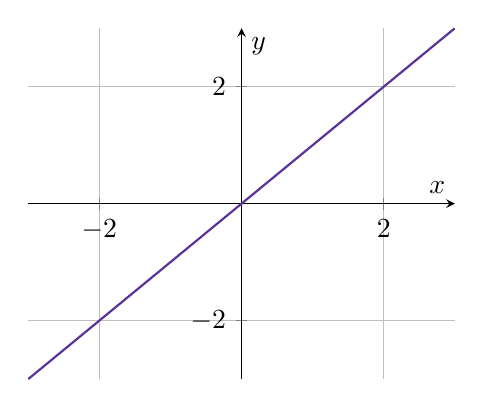
\begin{tikzpicture}
    \begin{axis}[
        grid=both,
        axis lines=middle,
        xmin=-3, xmax=3,
        ymin=-3, ymax=3,
        xlabel={$x$},
        ylabel={$y$},
        ]
        \addplot[RoyalPurple, thick, domain=-3:3] {x};
    \end{axis}
\end{tikzpicture}
\end{minipage}
\hspace{1cm}
\begin{minipage}{0.4\textwidth}
\centering
\begin{tabular}{cc}

$x$ & $f(x)$ \\
-2 & -2 \\
-1 & -1 \\
0 & 0 \\
1 & 1 \\
2 & 2 \\

\end{tabular}
\end{minipage}

The linear function $f(x) = x$ represents a \hl{straight line} that passes through the origin (0,0) and has a slope of 1. As $x$ increases or decreases, $f(x)$ increases or decreases respectively.

\subsection*{2. Quadratic Function: $f(x) = x^2$}
\begin{minipage}{0.5\textwidth}
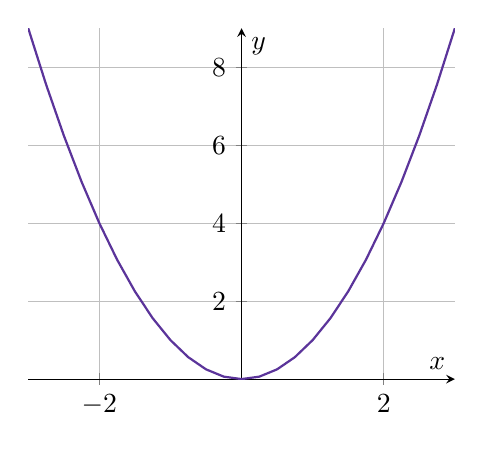
\begin{tikzpicture}
    \begin{axis}[
        grid=both,
        axis lines=middle,
        xmin=-3, xmax=3,
        ymin=0, ymax=9,
        xlabel={$x$},
        ylabel={$y$},
        ]
        \addplot[RoyalPurple, thick, domain=-3:3] {x^2};
    \end{axis}
\end{tikzpicture}
\end{minipage}
\hspace{1cm}
\begin{minipage}{0.4\textwidth}
\centering
\begin{tabular}{cc}
\toprule
$x$ & $f(x)$ \\

-2 & 4 \\
-1 & 1 \\
0 & 0 \\
1 & 1 \\
2 & 4 \\

\end{tabular}
\end{minipage}

The quadratic function $f(x) = x^2$ represents a parabola that opens upwards and has \hl{its vertex} at the origin (0,0). The function values are always non-negative and increase quadratically as $x$ moves away from 0.

\subsection*{3. Cubic Function: $f(x) = x^3$}
\begin{minipage}{0.5\textwidth}
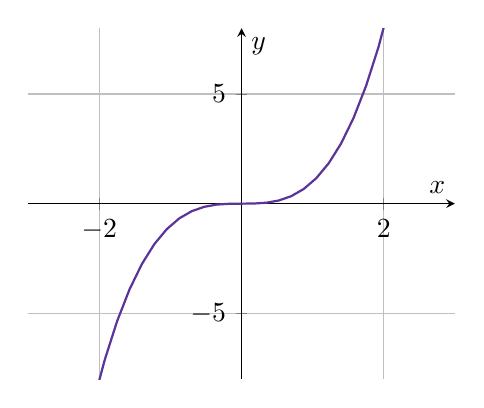
\begin{tikzpicture}
    \begin{axis}[
        grid=both,
        axis lines=middle,
        xmin=-3, xmax=3,
        ymin=-8, ymax=8,
        xlabel={$x$},
        ylabel={$y$},
        ]
        \addplot[RoyalPurple, thick, domain=-2.1:2.1] {x^3};
    \end{axis}
\end{tikzpicture}
\end{minipage}
\hspace{1cm}
\begin{minipage}{0.4\textwidth}
\centering
\begin{tabular}{cc}

$x$ & $f(x)$ \\

-2 & -8 \\
-1 & -1 \\
0 & 0 \\
1 & 1 \\
2 & 8 \\
\end{tabular}
\end{minipage}

The cubic function $f(x) = x^3$ has a characteristic \hl{S-shape} and crosses the origin (0,0). The function values increase cubically as $x$ moves away from 0, with $f(x)$ being negative when $x$ is negative and positive when $x$ is positive.

\subsection*{4. Reciprocal Function: $f(x) = \frac{1}{x}$}
\begin{minipage}{0.5\textwidth}
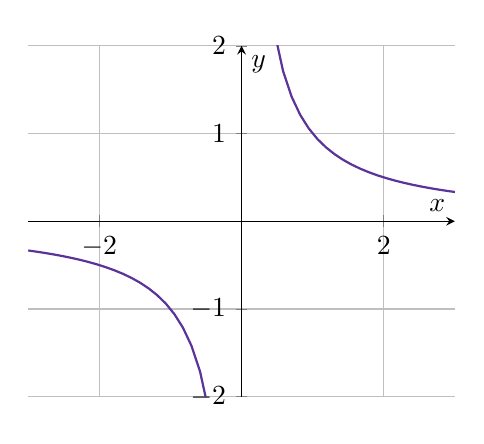
\begin{tikzpicture}
    \begin{axis}[
        grid=both,
        axis lines=middle,
        xmin=-3, xmax=3,
        ymin=-2, ymax=2,
        xlabel={$x$},
        ylabel={$y$},
        ]
        \addplot[RoyalPurple, thick, domain=-3:-0.1] {1/x};
        \addplot[RoyalPurple, thick, domain=0.1:3] {1/x};
    \end{axis}
\end{tikzpicture}
\end{minipage}
\hspace{1cm}
\begin{minipage}{0.4\textwidth}
\centering
\begin{tabular}{cc}

$x$ & $f(x)$ \\

-3 & -0.33 \\
-2 & -0.5 \\
-1 & -1 \\
1 & 1 \\
2 & 0.5 \\
3 & 0.33 \\

\end{tabular}
\end{minipage}
\noindent
The reciprocal function $f(x) = \frac{1}{x}$ has \hl{two hyperbolas} in the 1st and 3rd quadrants. As $x$ approaches 0 from either side, $f(x)$ approaches $\pm\infty$. 

\subsection*{5. Square Root Function: $f(x) = \sqrt{x}$}
\begin{minipage}{0.5\textwidth}
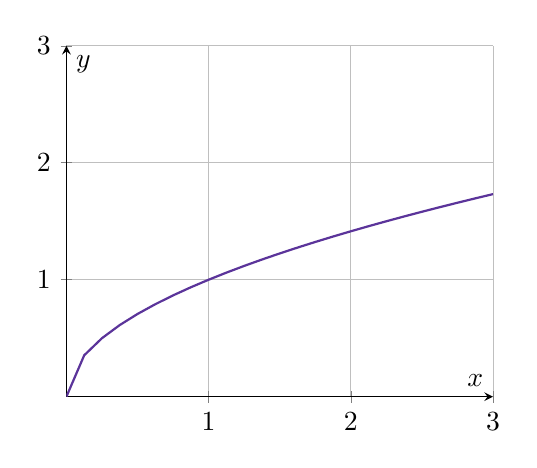
\begin{tikzpicture}
    \begin{axis}[
        grid=both,
        axis lines=middle,
        xmin=0, xmax=3,
        ymin=0, ymax=3,
        xlabel={$x$},
        ylabel={$y$},
        ]
        \addplot[RoyalPurple, thick, domain=0:3] {sqrt(x)};
    \end{axis}
\end{tikzpicture}
\end{minipage}
\hspace{1cm}
\begin{minipage}{0.4\textwidth}
\centering
\begin{tabular}{cc}
\toprule
$x$ & $f(x)$ \\

0 & 0 \\
1 & 1 \\
2 & 1.41 \\
3 & 1.73 \\

\end{tabular}
\end{minipage}
\noindent
The square root function $f(x) = \sqrt{x}$ is defined for $x \geq 0$ and represents \hl{half of a parabola} that opens upwards. As $x$ increases, $f(x)$ increases more slowly.


\subsection*{6. Absolute Value Function: $f(x) = |x|$}
\begin{minipage}{0.5\textwidth}
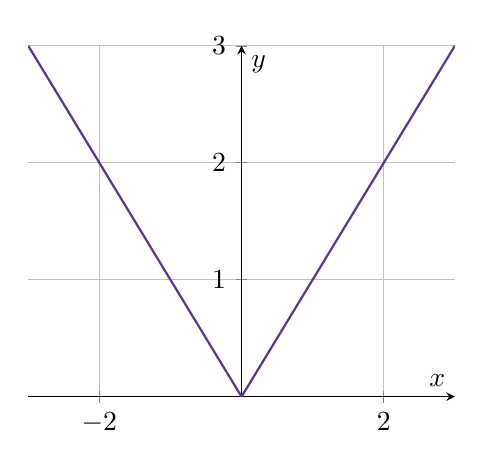
\begin{tikzpicture}
    \begin{axis}[
        grid=both,
        axis lines=middle,
        xmin=-3, xmax=3,
        ymin=0, ymax=3,
        xlabel={$x$},
        ylabel={$y$},
        ]
        \addplot[RoyalPurple, thick, domain=-3:3] {abs(x)};
    \end{axis}
\end{tikzpicture}
\end{minipage}
\hspace{1cm}
\begin{minipage}{0.4\textwidth}
\centering
\begin{tabular}{cc}

$x$ & $f(x)$ \\

-2 & 2 \\
-1 & 1 \\
0 & 0 \\
1 & 1 \\
2 & 2 \\

\end{tabular}
\end{minipage}
\noindent
The absolute value function $f(x) = |x|$ represents a \hl{V-shaped graph} that has its vertex at the origin (0,0). The function values are always non-negative, regardless of the sign of $x$.\\
\end{document}